\documentclass[aspectratio=169]{beamer}
\setbeamertemplate{navigation symbols}{}
\usepackage{color,amsmath,comment, subfigure}
\usepackage{booktabs}
\usepackage{url}

%\setbeameroption{show notes}

%%%%%%%%%%%%%%%%%%%%%%%%%%
\title[]{Class 8: Spread of disease in networks}
\author[]{Matthew J. Salganik}
\institute[]{Sociology 204: Social Networks, Spring 2021\\Princeton University}
\date[]{
1/3: Spread of disease
\vfill 

\begin{flushleft}
\vspace{0.6in}

\includegraphics[width=0.1\textwidth]{figures/cc.png}
\end{flushleft}

}

\note{
TODO: Move candy bowl to the end of this class possibly. Helps set the stage for next class and has them do it before they see the readings
TODO: Try to find movie of chains of affection
}

\begin{document}
%%%%%%%%%%%%%%%%%%%%%%%%%%%
\frame{\titlepage}
%%%%%%%%%%%%%%%%%%%%%%%%%%%
\begin{comment}
\begin{frame}

SWBAT:
\begin{enumerate}
\end{enumerate}

\end{frame}
\end{comment}
%%%%%%%%%%%%%%%%%%%%%%%%
\begin{frame}

\begin{itemize}
\item directed search and broadcast search
\pause
\item how is directed search possible
\pause
\item example of directed search: search for an abortionist
\end{itemize}

\pause
Today: broadcast search because that's what diseases use

\end{frame}
%%%%%%%%%%%%%%%%%%%%%%%%%
\begin{frame}

\begin{figure}
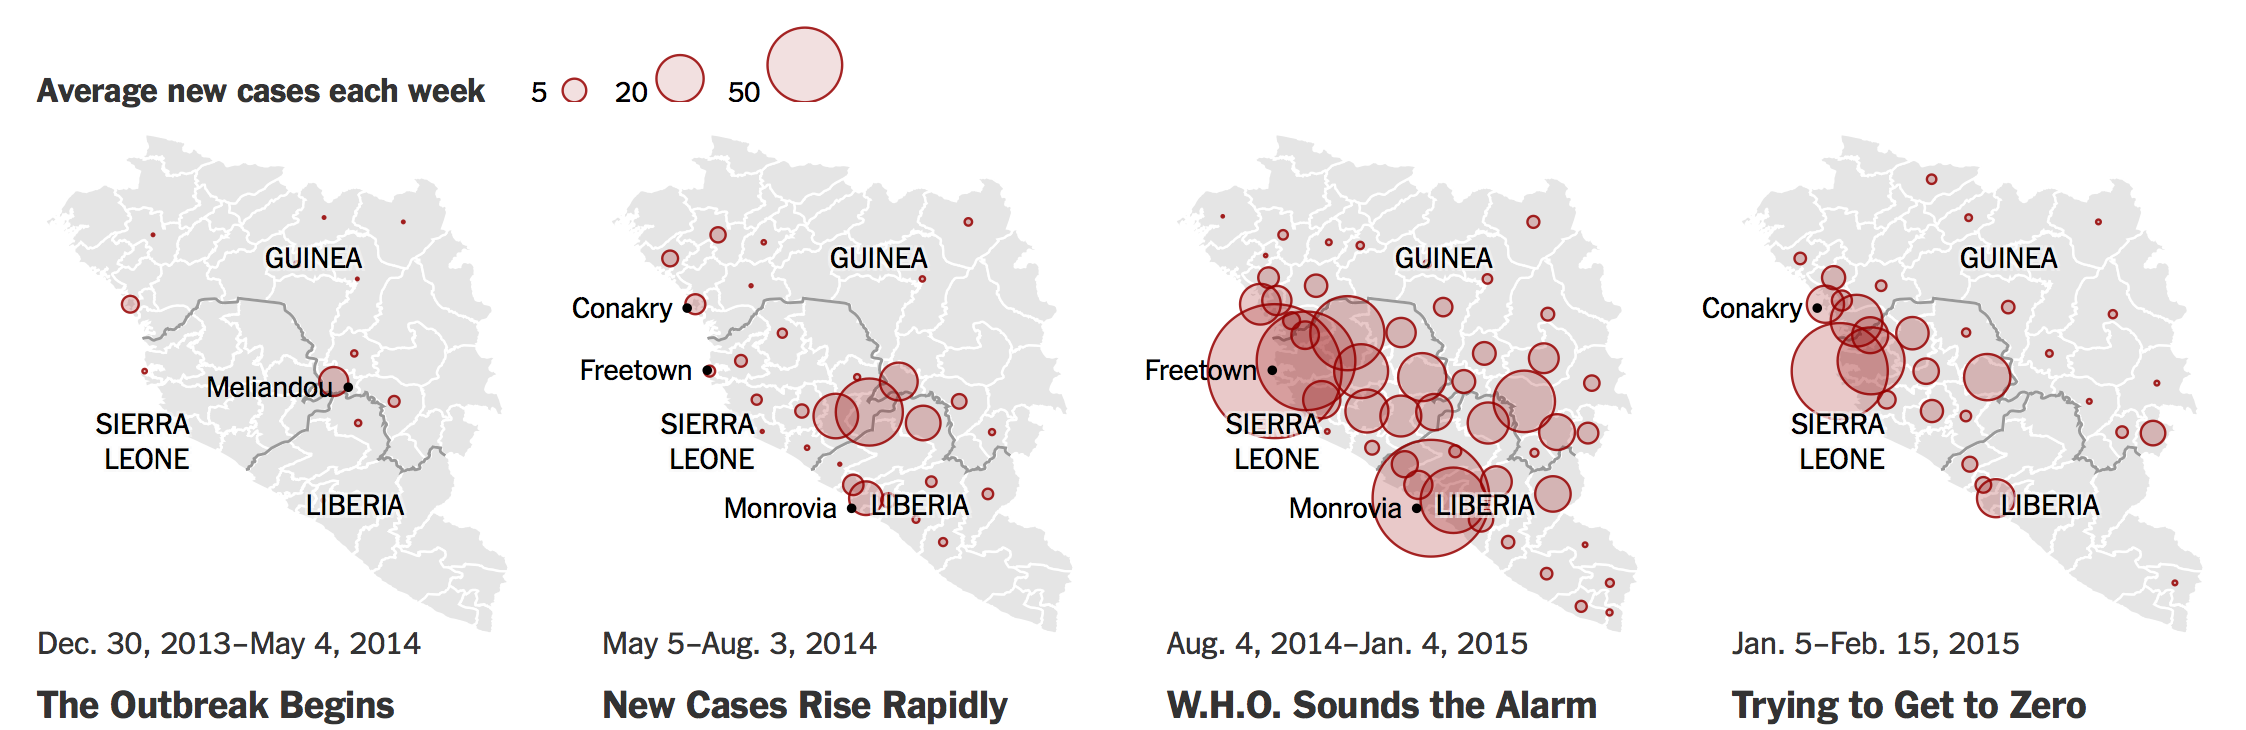
\includegraphics[width=0.95\textwidth]{figures/ebola_maps}
\end{figure}

\tiny{\url{http://www.nytimes.com/interactive/2015/02/24/world/africa/2015-02-24-ebola-outbreak.html}}

\note{
This is what Duncan warned us about

What if Ebola gets to a big city?
}

\end{frame}
%%%%%%%%%%%%%%%%%%%%%%%%%
%\begin{frame}
%
%\begin{center}
%Chains of transmission and control of Ebola Virus Disease in Conakry, Guinea in 2014\\
%by Simon Cauchemez\\
%Mathematical Modelling of Infectious Diseases Unit\\
%Institut Pasteur, Paris\\
%\end{center}
%
%Speaking at Princeton University February 24, 2015
%\note{
%Here are slides from Simon's talk.  What happens when Ebola gets into an urban center?
%}
%
%\end{frame}
%%%%%%%%%%%%%%%%%%%%%%%%%%
%\begin{frame}
%
%\begin{figure}
%
\includegraphics[width=0.95\textwidth]{figures/email_to_simon}
%\end{figure}
%
%\end{frame}
%%%%%%%%%%%%%%%%%%%%%%%%%%
\begin{frame}

\begin{figure}
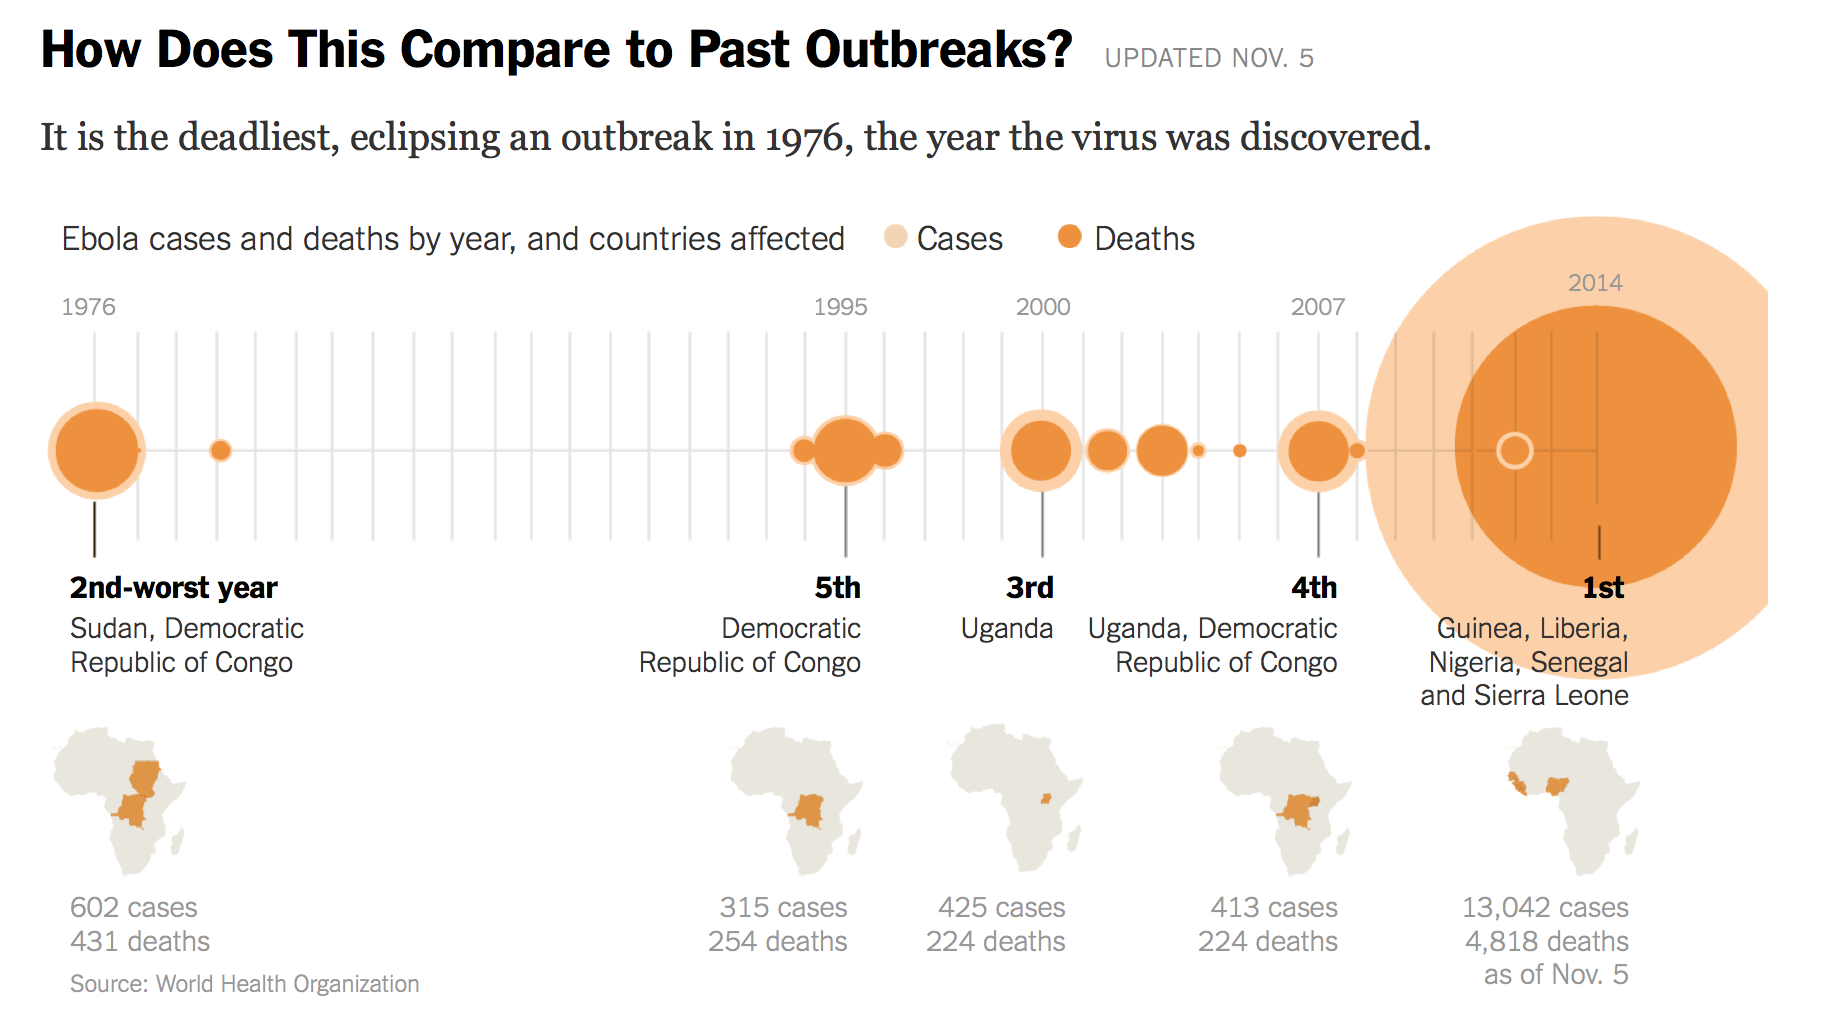
\includegraphics[width=0.95\textwidth]{figures/ebola_timeline}
\end{figure}

\tiny{\url{http://www.nytimes.com/interactive/2014/07/31/world/africa/ebola-virus-outbreak-qa.html}}

\note{

}

\end{frame}
%%%%%%%%%%%%%%%%%%%%%%%%%%
\begin{frame}

\begin{figure}
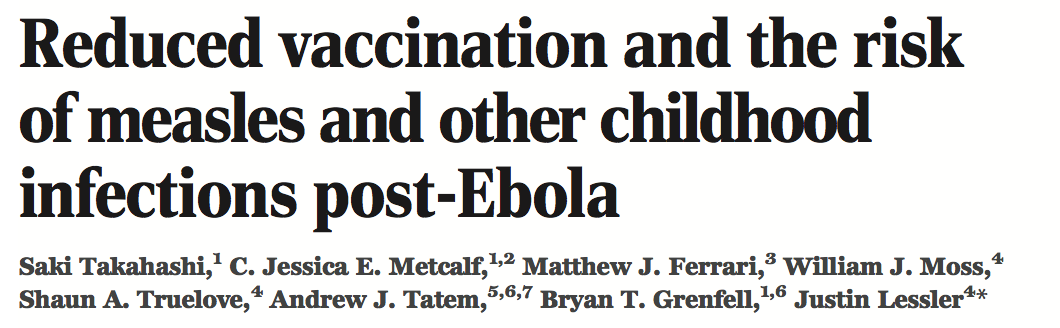
\includegraphics[width=0.95\textwidth]{figures/takahashi_reduced_2015_title}
\end{figure}

\vfill

\url{http://dx.doi.org/10.1126/science.aaa3438}

\note{
Diseases can have long-term impacts in unexpected ways.  People stop getting vaccines can lead to outbreaks of disease in the future

}

\end{frame}
%%%%%%%%%%%%%%%%%%%%%%%%%%
\begin{frame}

What does the future of global pandemics look like?  Is technology going to help us or hurt us?

\note{
Medical knowledge will increase but now virus can get on an airplane
}

\end{frame}
%%%%%%%%%%%%%%%%%%%%%%%%%%
\begin{frame}

\begin{figure}
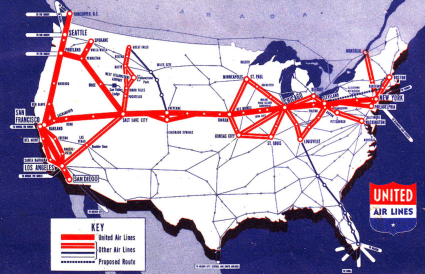
\includegraphics[width=0.8\textwidth]{figures/UAL_Route_Map_1940}
\end{figure}

\tiny{\url{http://en.wikipedia.org/wiki/United_Airlines\#mediaviewer/File:UAL_Route_Map_1940.jpg}}

\end{frame}
%%%%%%%%%%%%%%%%%%%%%%%%%%%
\begin{frame}

\begin{figure}
\includegraphics[width=0.8\textwidth]{figures/UAL_NA_Map_2015_02_01}
\end{figure}

\tiny{\url{http://www.united.com/CMS/Documents/pdfs/route-maps/UAL_NA_Map_2015_02_01.pdf}}

\end{frame}
%%%%%%%%%%%%%%%%%%%%%%%%%%%
\begin{frame}

\begin{figure}
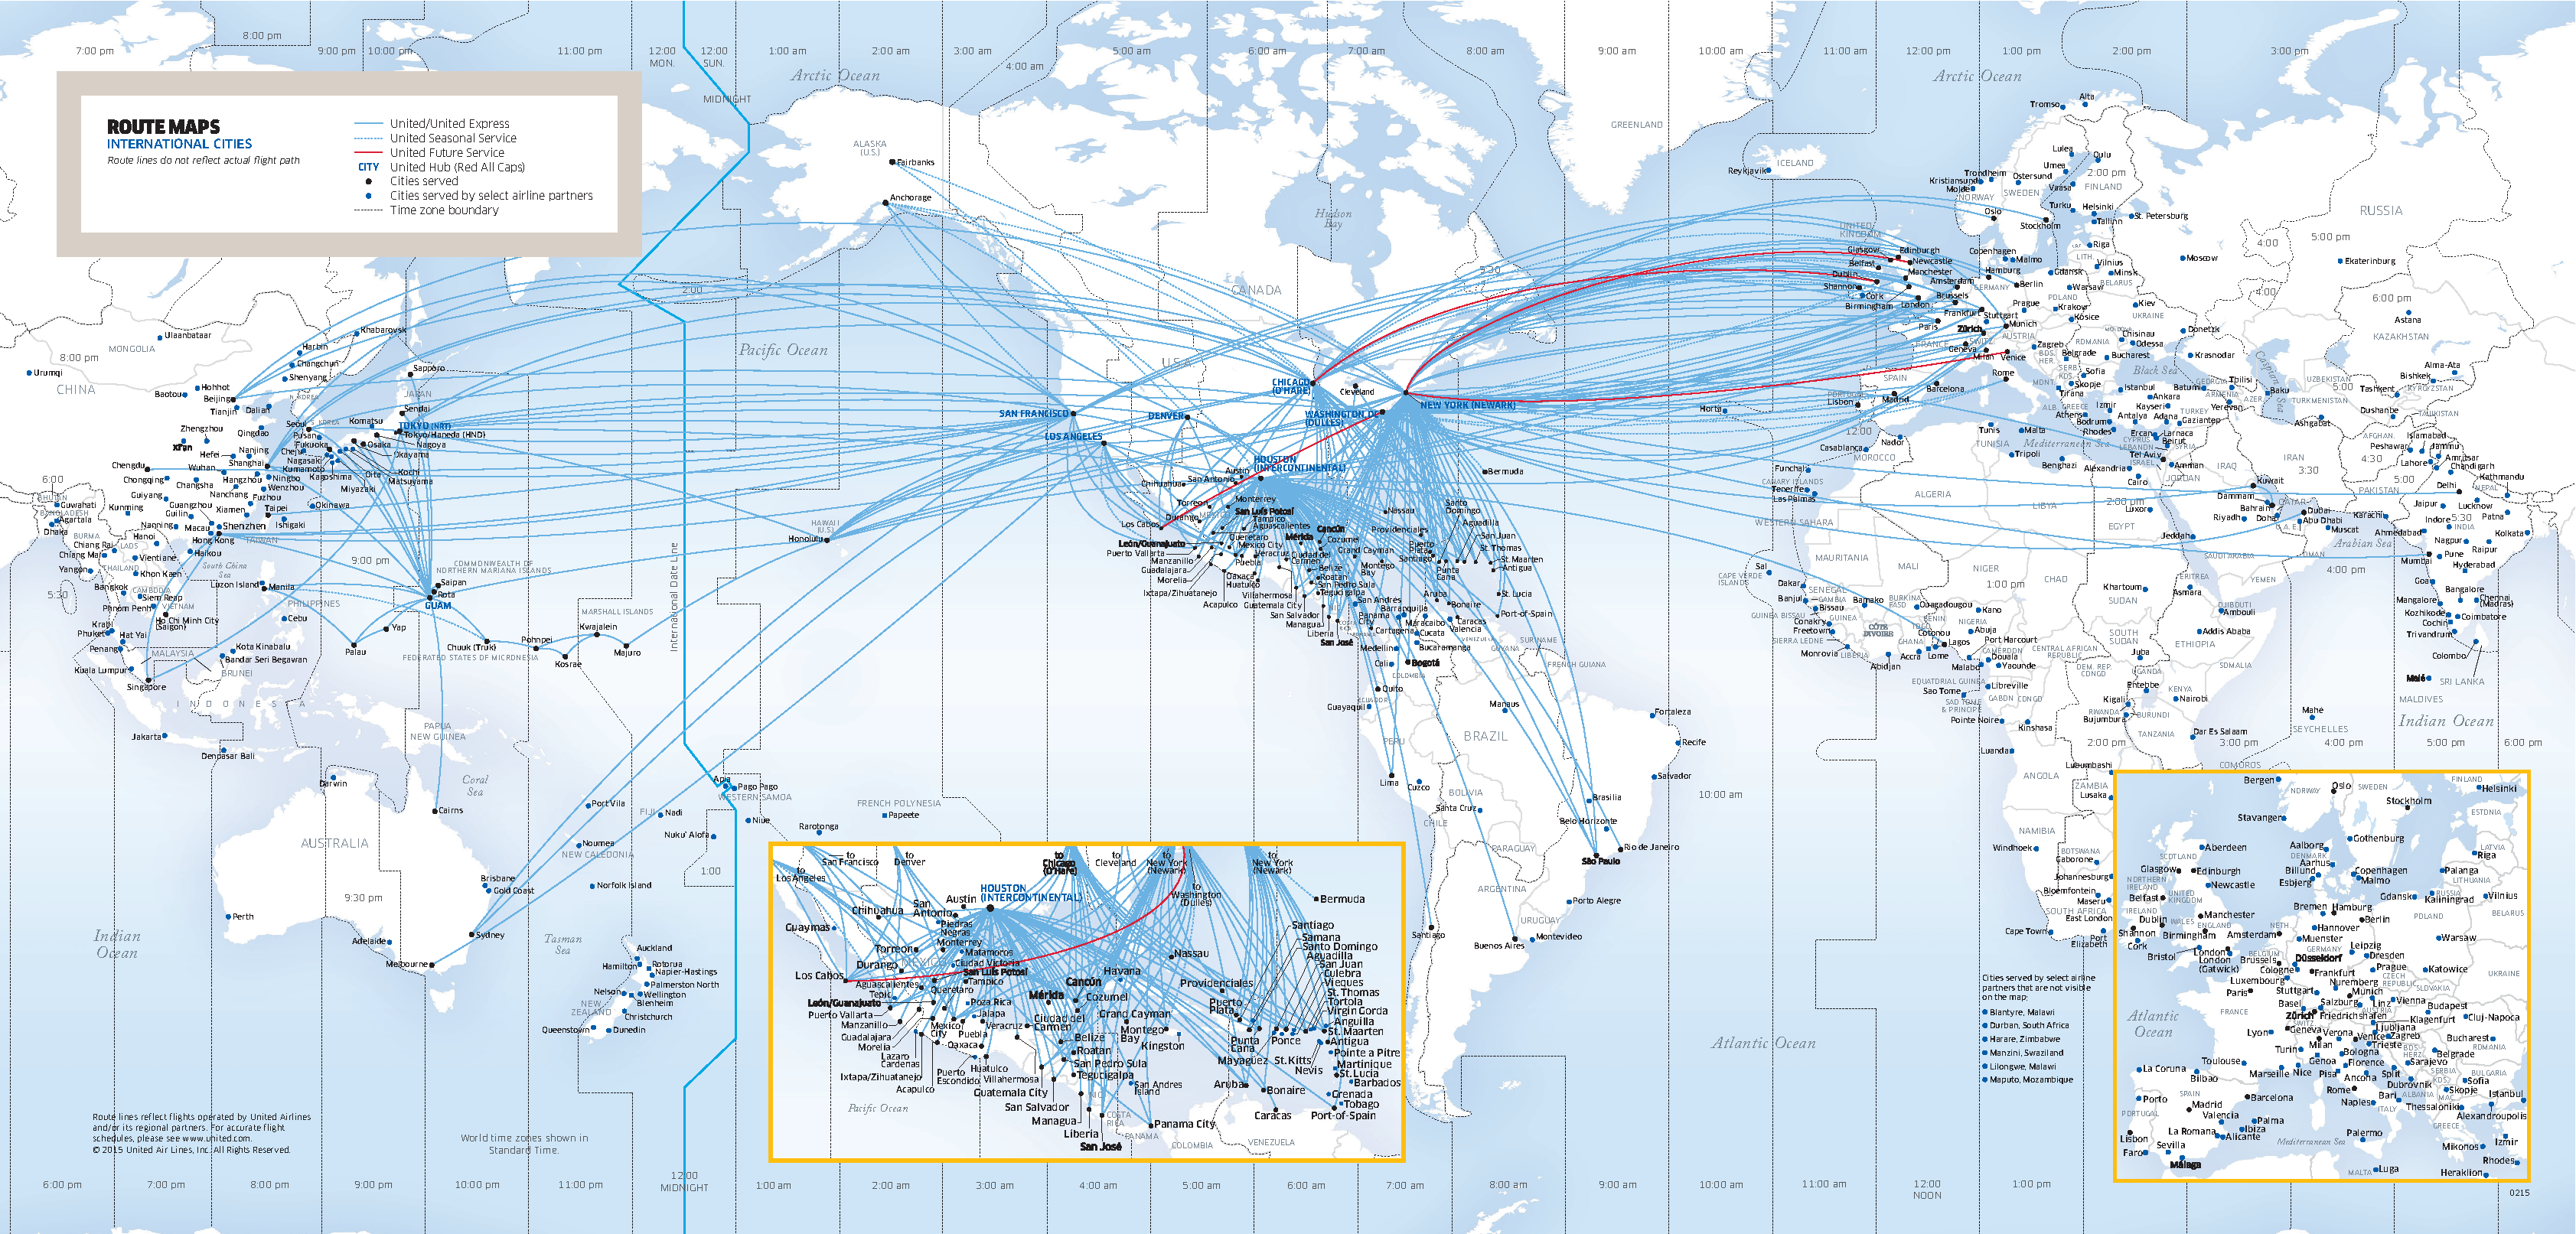
\includegraphics[width=0.8\textwidth]{figures/UAL_WORLD_Map_2015_02_01}
\end{figure}

\tiny{\url{http://www.united.com/CMS/Documents/pdfs/route-maps/UAL_WORLD_Map_2015_02_01.pdf}}

\note{

Note the similarity to computer viruses that Duncan mentions.  Global computer virus is helped by connectivity of the internet

}

\end{frame}
%%%%%%%%%%%%%%%%%%%%%%%%
\begin{frame}

Is technology going to help or hurt with the next global pandemic?
\begin{enumerate}
\item help
\item hurt
\end{enumerate}

\note{
Depends on the disease. for example travel is especially bad for diseases with long incubation period and asymptomatic spread

}

\end{frame}
%%%%%%%%%%%%%%%%%%%%%%%%%%%
\begin{frame}

Main tools for thinking about epidemics:
\begin{itemize}
\item $R_0$
\item SIR model
\end{itemize}

\note{
}

\end{frame}
%%%%%%%%%%%%%%%%%%%%%%%%%%%
\begin{frame}

\begin{itemize}
\item $R_0$: Number of new cases when a disease is introduced into a fully susceptible population
\pause
\item $R$: Reproduction rate: the average number of new infections generated by each currently infected individual 
\end{itemize}

\note{
}

\end{frame}
%%%%%%%%%%%%%%%%%%%%%%%%%%
\begin{frame}

\begin{center}
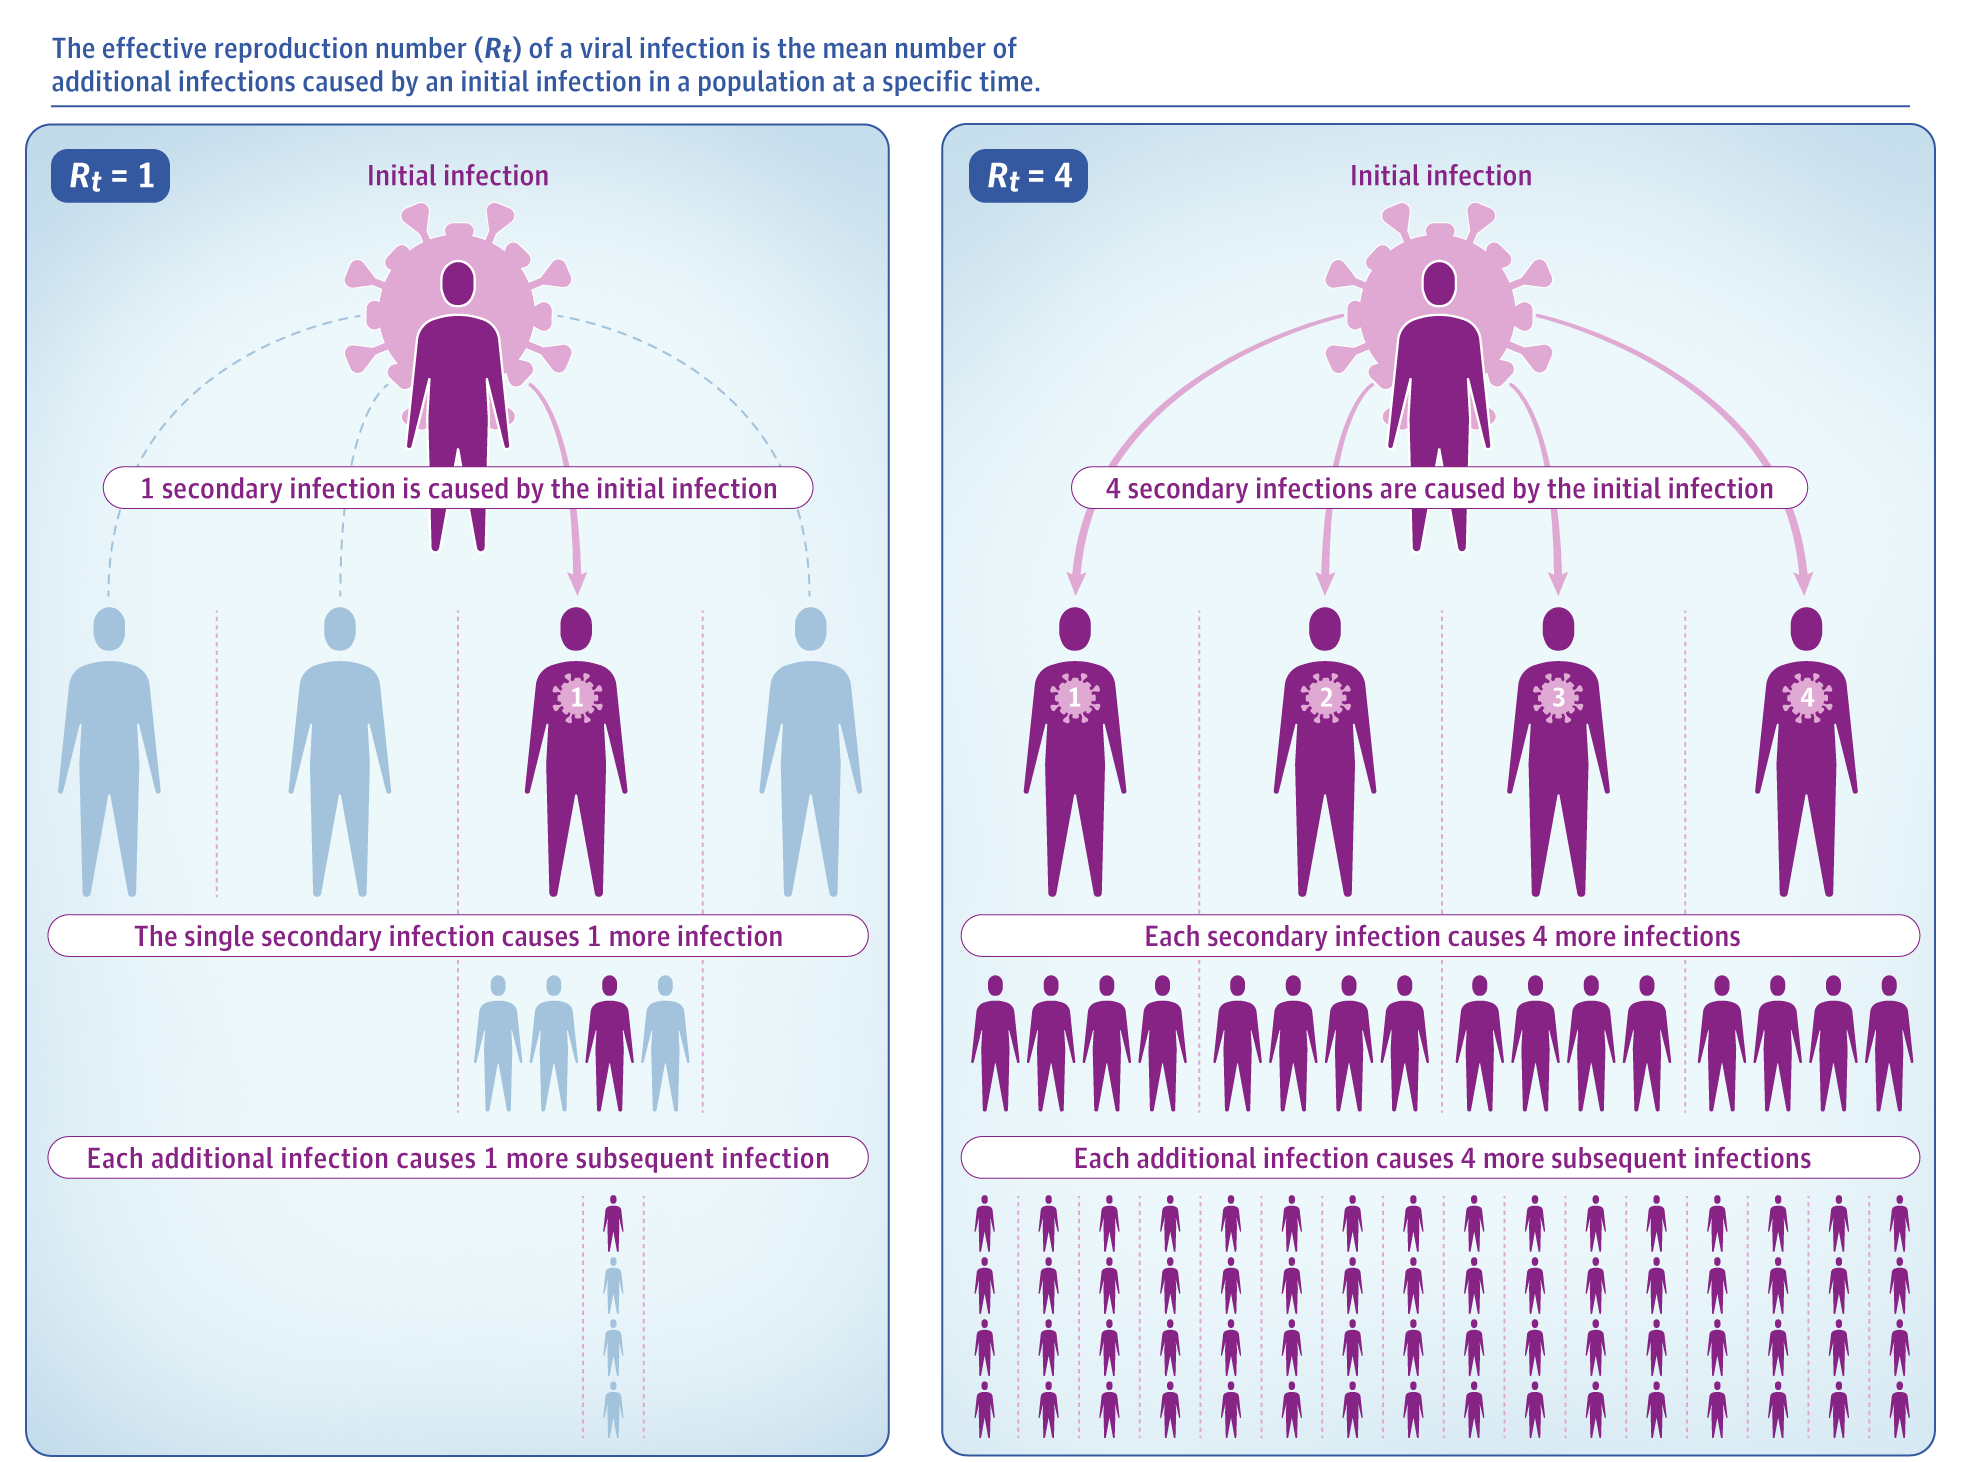
\includegraphics[height = 0.90\textheight]{figures/inglesby_public_2020_fig1}
\end{center}

\vfill
\url{http://dx.doi.org/10.1001/jama.2020.7878}
\end{frame}
%%%%%%%%%%%%%%%%%%%%%%%%%
\begin{frame}

R can vary of space and time

\url{http://metrics.covid19-analysis.org/}

\end{frame}
%%%%%%%%%%%%%%%%%%%%%%%%%% 
\begin{frame}

Main tools for thinking about epidemics:
\begin{itemize}
\item $R_0$
\item SIR model
\end{itemize}

\note{
}

\end{frame}
%%%%%%%%%%%%%%%%%%%%%%%%%%%
\begin{frame}

\begin{center}
\includegraphics[width = 0.90\textwidth]{figures_book/6_1}
\end{center}

\end{frame}
%%%%%%%%%%%%%%%%%%%%%%%%%%%%
\begin{frame}

$R \texttt{ in SIR model } \ne R_0 \ne R$

\end{frame}
%%%%%%%%%%%%%%%%%%%%%%%%%%%%
\begin{frame}

\begin{center}
\includegraphics[width = 0.90\textwidth]{figures_book/6_2}
\end{center}

\note{
No network structure
}


\end{frame}
%%%%%%%%%%%%%%%%%%%%%%%%%%%%
\begin{frame}

\begin{center}
\includegraphics[width = 0.80\textwidth]{figures_book/6_3}
\end{center}

\end{frame}
%%%%%%%%%%%%%%%%%%%%%%%%%%%%
\begin{frame}

\begin{center}
\includegraphics[width = 0.80\textwidth]{figures_book/6_4}
\end{center}

\end{frame}
%%%%%%%%%%%%%%%%%%%%%%%%%%%%
\begin{frame}

What shape will the Ebola time series have?

\end{frame}
%%%%%%%%%%%%%%%%%%%%%%%%%%%
\begin{frame}

\begin{center}
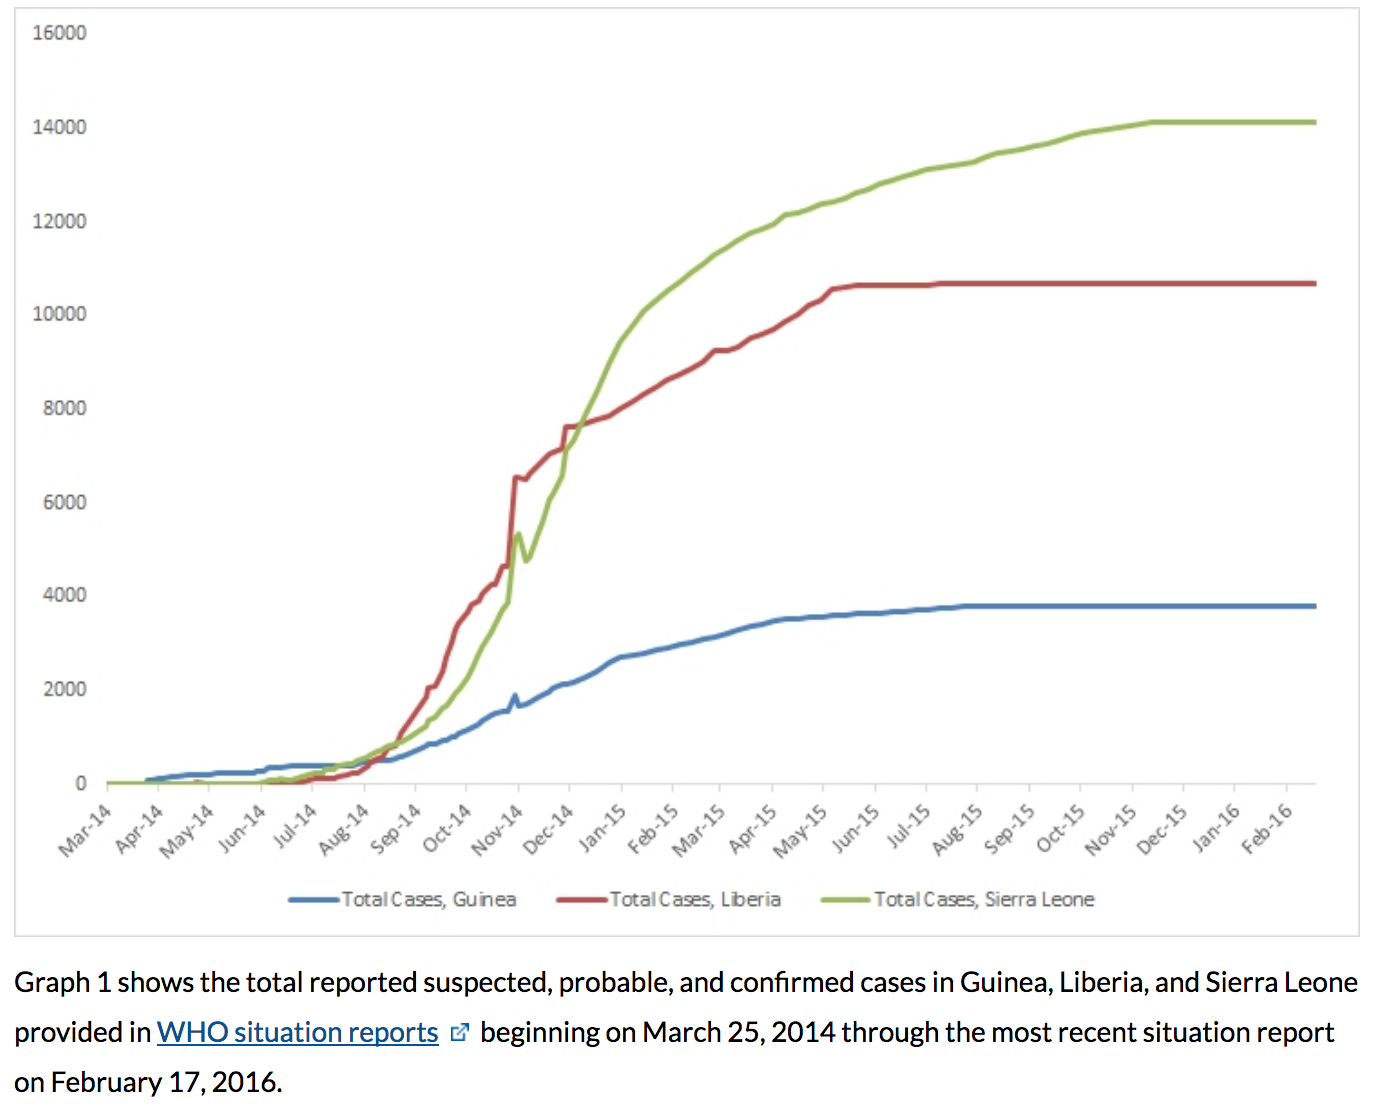
\includegraphics[width = 0.7\textwidth]{figures/ebola_timeseries}
\end{center}

\vfill

\url{https://www.cdc.gov/vhf/ebola/outbreaks/2014-west-africa/cumulative-cases-graphs.html}

\note{
This looks like the S shaped curve that Watts talked about
Is this 3 epidemics or 1 epidemic?

What the SIR model does not tell us in N.  How many people will be infected?
}

\end{frame}
%%%%%%%%%%%%%%%%%%%%%%%%%%%
\begin{frame}

Relationship between networks and disease

\end{frame}
%%%%%%%%%%%%%%%%%%%%%%%%%%%
\begin{frame}

\begin{center}
\includegraphics[width = 0.95\textwidth]{figures_book/3_6}
\end{center}

\note{
spread of diseases on a small world graph

with no rewiring we disease fronts and slow spread

at randomly mixed limit we have SIR model fast spread

In the middle we have low path length like 

focus on the shortcuts: in HIV this is often truck drivers, or shooting galleries
}

\end{frame}
%%%%%%%%%%%%%%%%%%%%%%%%%%%%%
\begin{frame}

\begin{center}
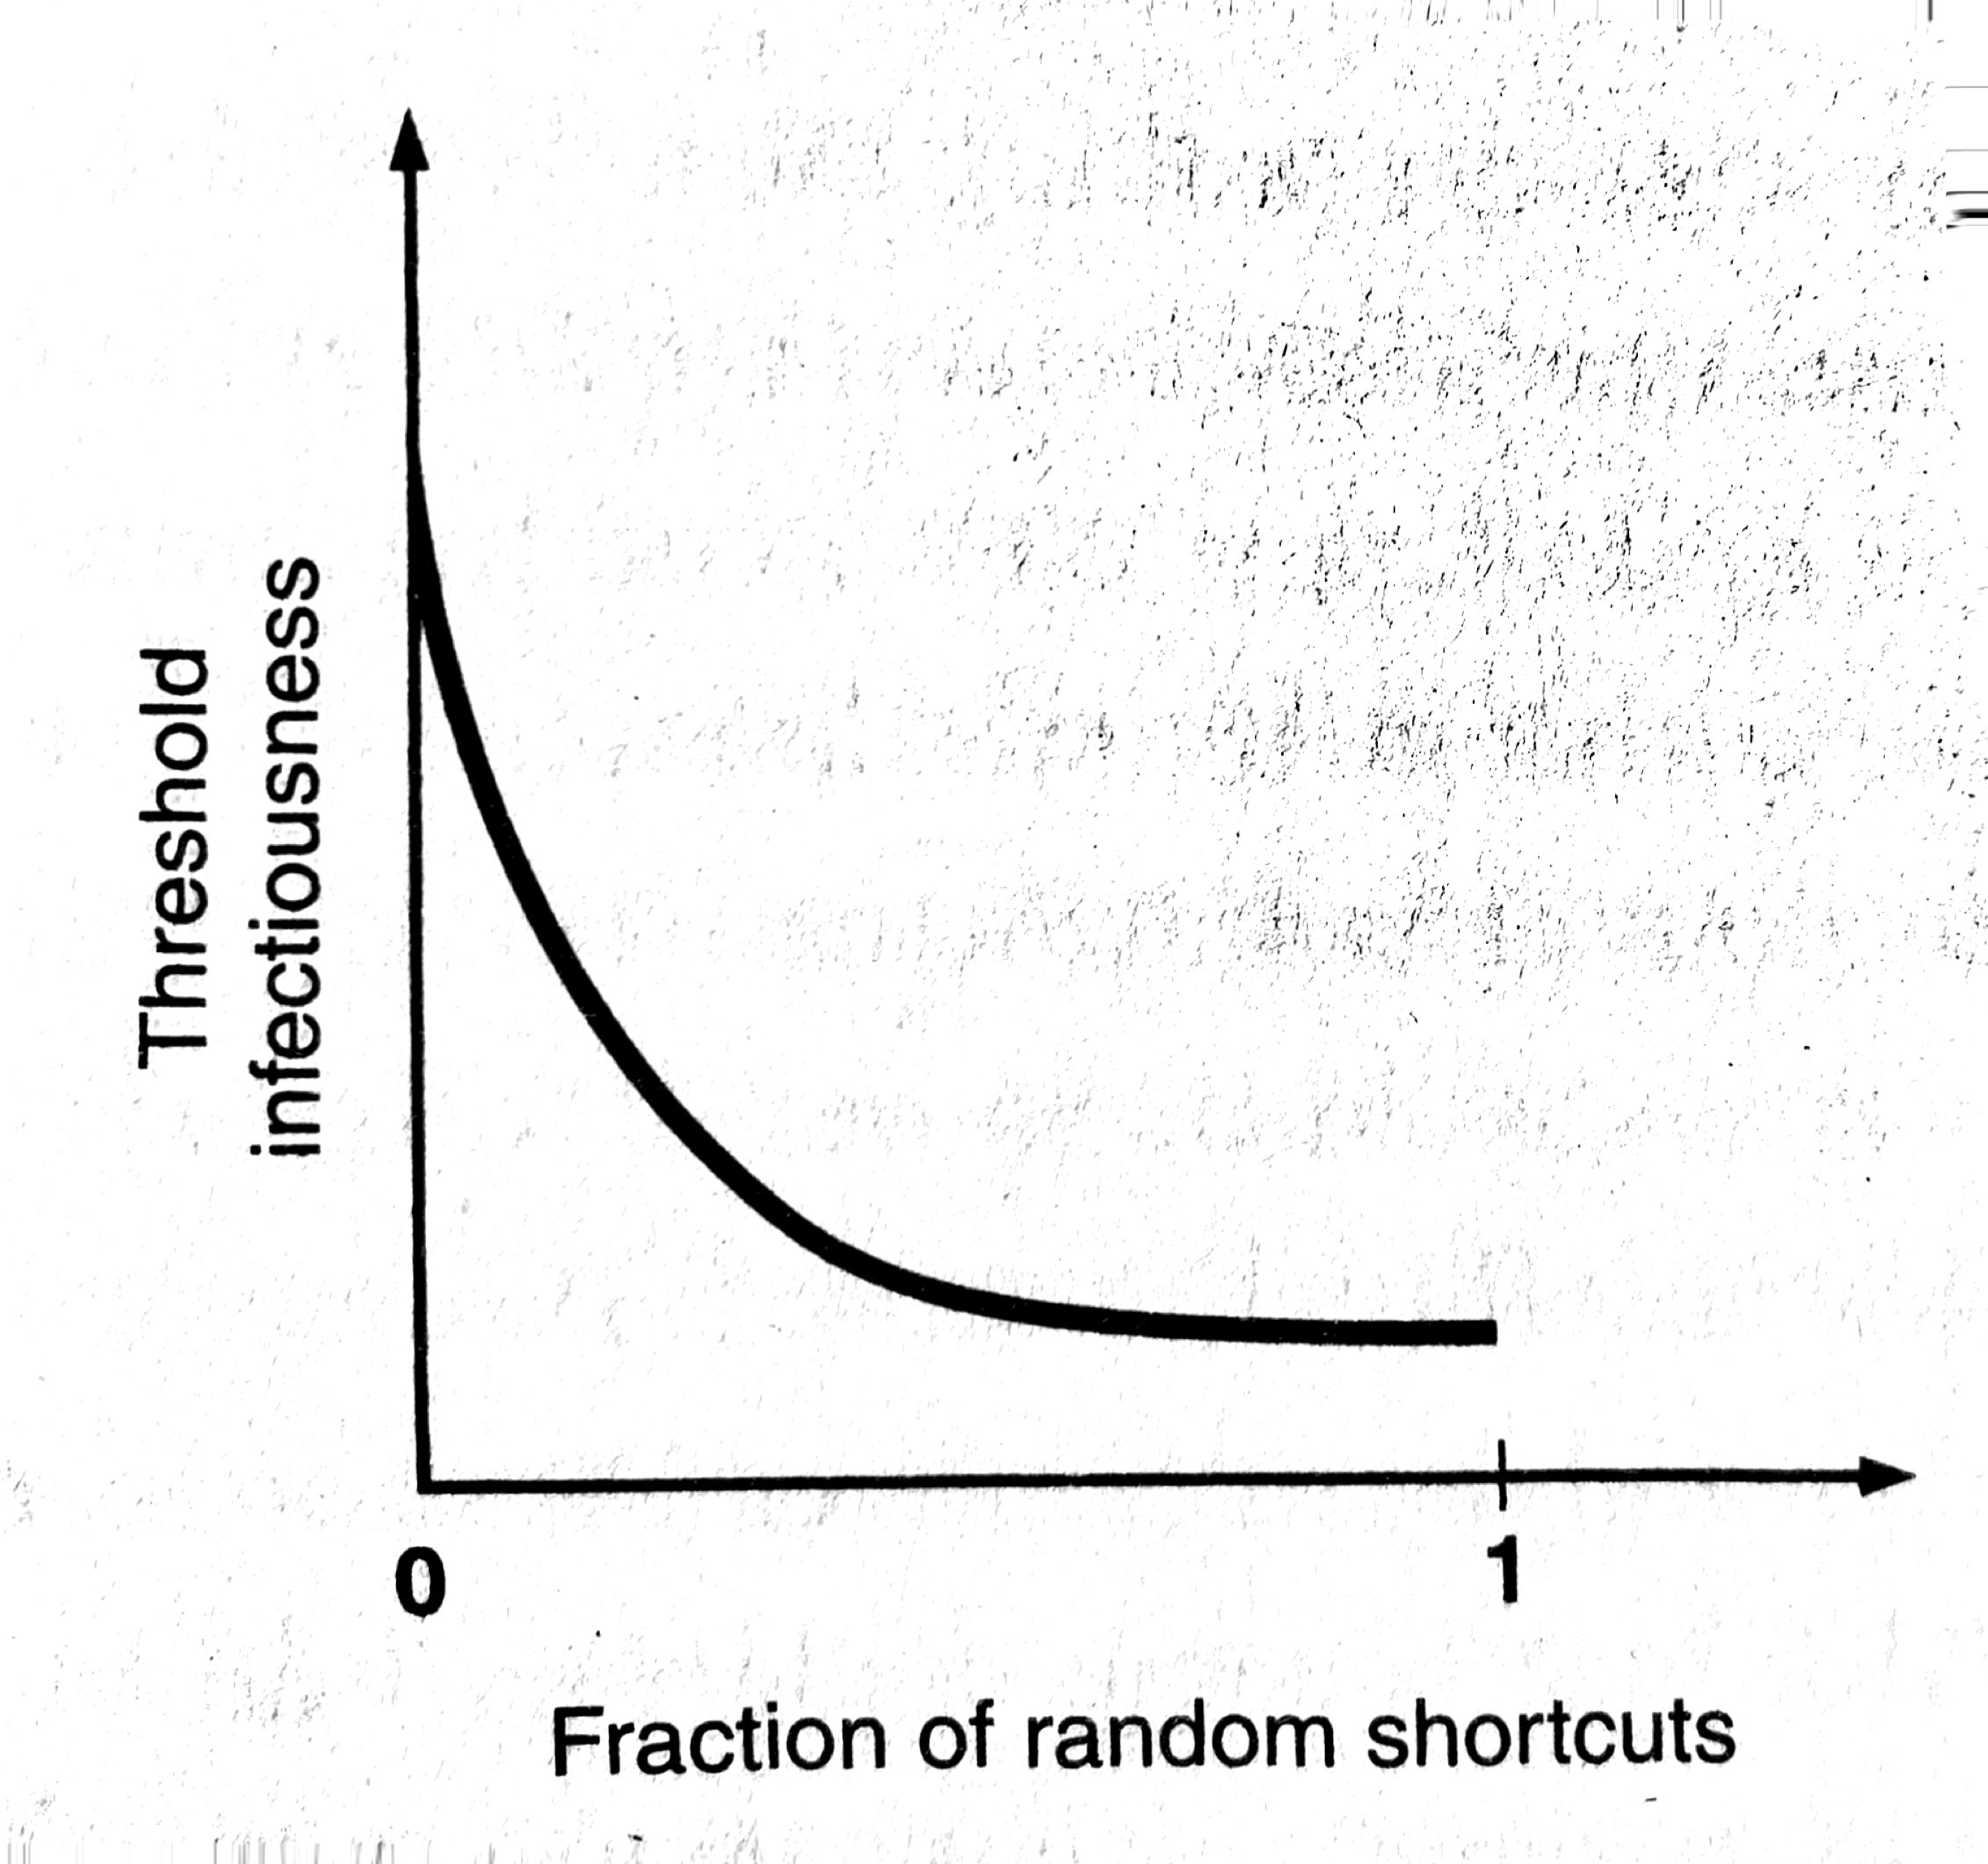
\includegraphics[width = 0.5\textwidth]{figures/6_9}
\end{center}

\note{
reduce shortcuts: less travel, policy targeted at short-cuts (e.g., truck drivers)
}

\end{frame}
%%%%%%%%%%%%%%%%%%%%%%%%%%%%%
\begin{frame}

\begin{center}

\includegraphics[width = 0.95\textwidth]{figures/marvel_small-world_2013_title}
\end{center}


\tiny{\url{http://arxiv.org/pdf/1310.2636v1.pdf}}

\note{

disease is also a probe into networks

}

\end{frame}
%%%%%%%%%%%%%%%%%%%%%%%%%%%%
\begin{frame}

\begin{center}
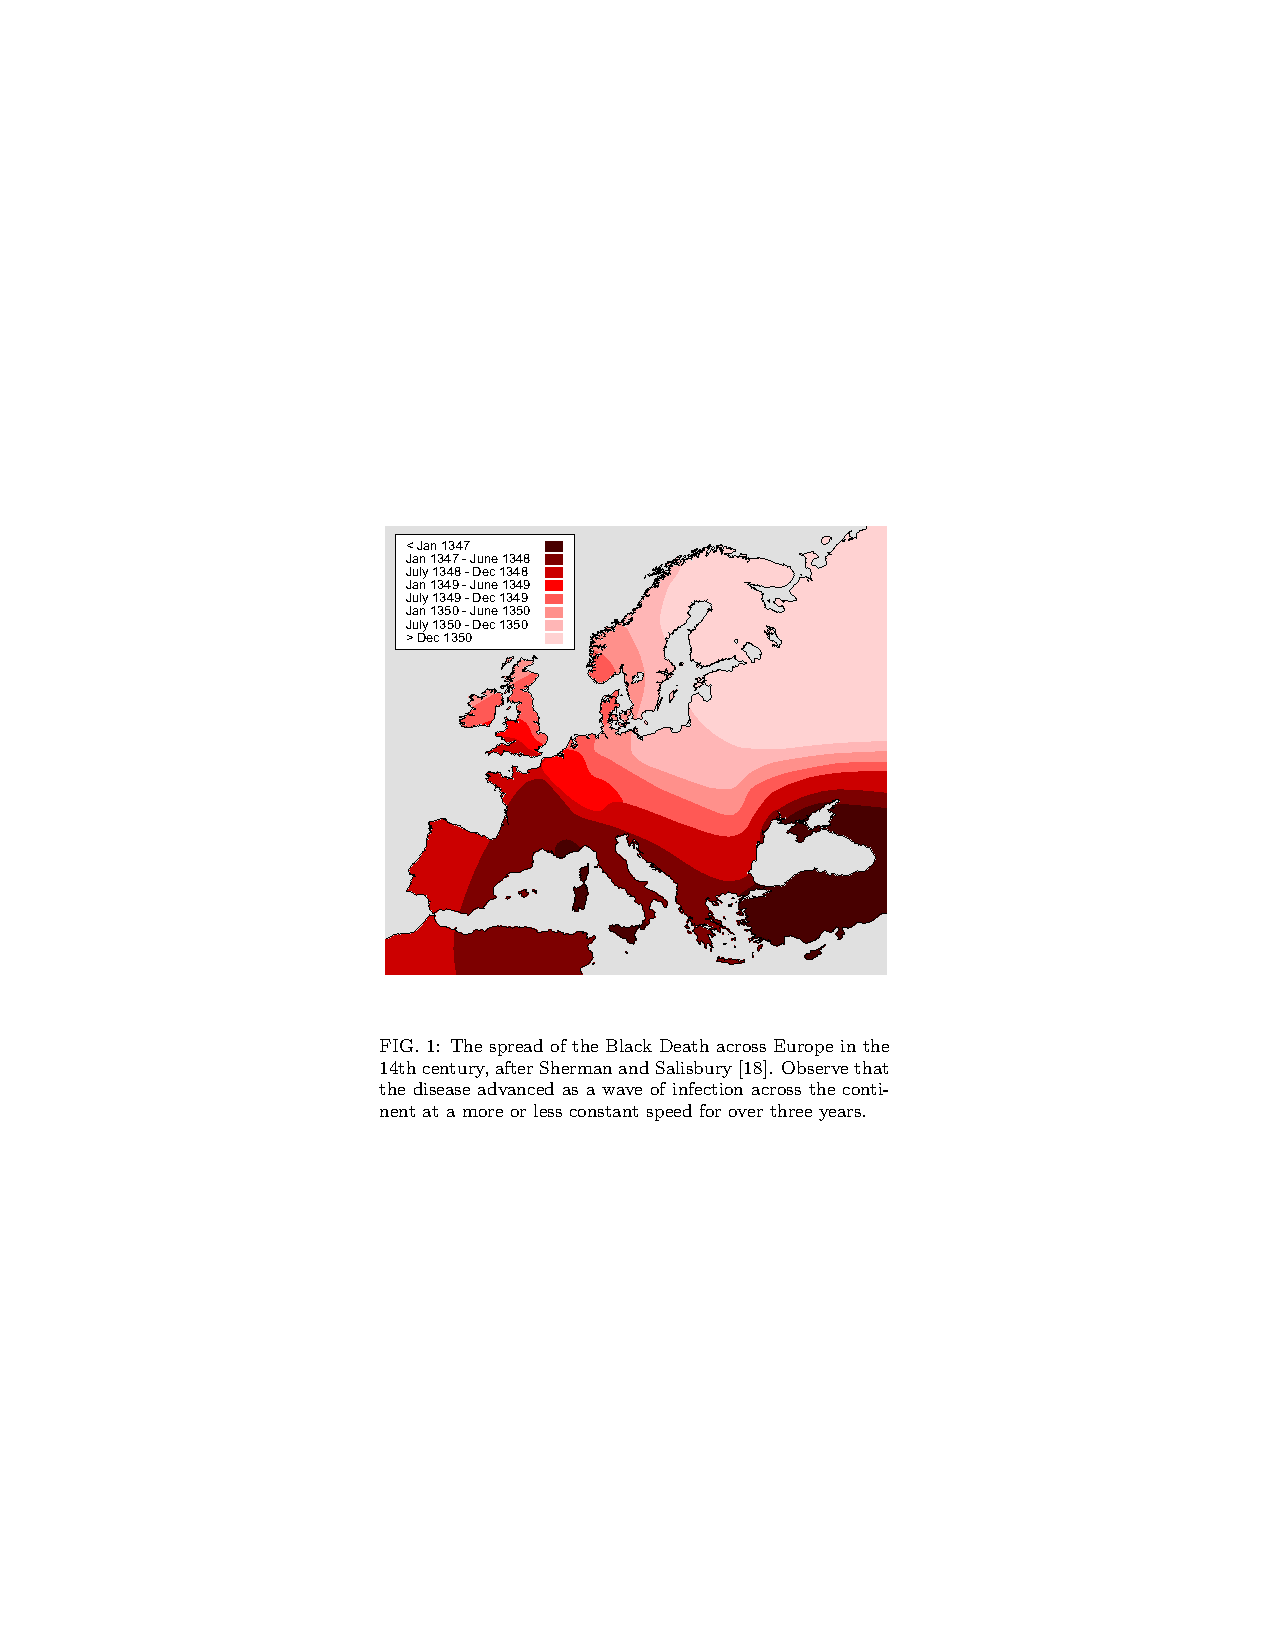
\includegraphics[width = 0.6\textwidth]{figures/marvel_small-world_2013_fig1}
\end{center}

\note{

slow spread of black death which was rats, fleas, and person to person
}

\end{frame}
%%%%%%%%%%%%%%%%%%%%%%%%%%%%
\begin{frame}

\begin{center}
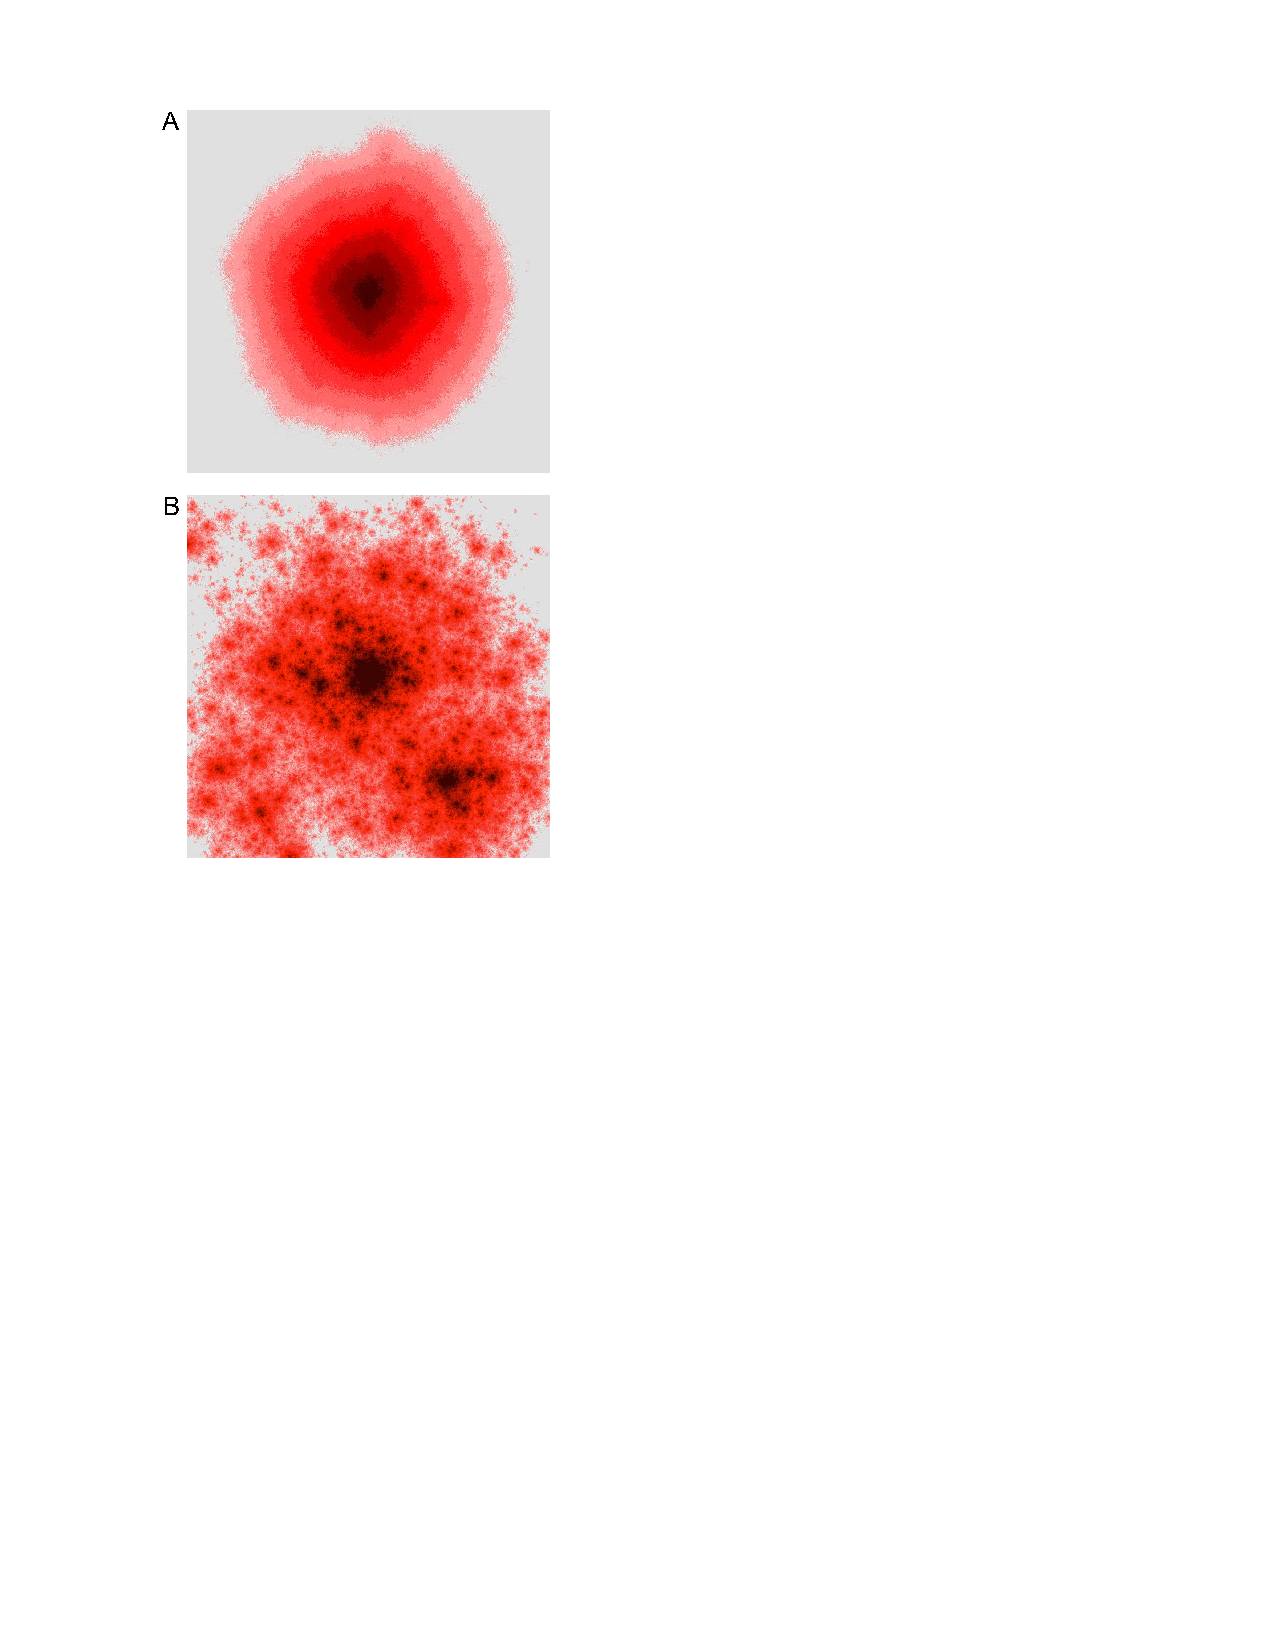
\includegraphics[height = 0.8\textheight]{figures/marvel_small-world_2013_fig2}
\end{center}

\vfill

\begin{itemize}
\item Top: Disease spread with no shortcuts
\item Bottom: Disease spread with long distance connections
\end{itemize}

\note{

top shows no long range connections

bottom shows with some long range connections

so spreads as if no long range contacts so implies no long range friendships implies no small world
}

\end{frame}
%%%%%%%%%%%%%%%%%%%%%%%%%%%%
\begin{frame}

Important to match the disease you are studying to the appropriate contact network.  For STDs, this is the sexual network.

Recall, this image of the sexual networks in Sweden.
\begin{center}
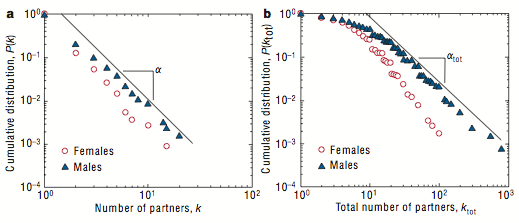
\includegraphics[width = 0.95\textwidth]{figures/liljeros_web_2001_fig2}
\end{center}

But what is the structure of sexual networks?

\note{

Degree distribution is not the whole sexual network

}

\end{frame}

\end{document}
